% Copyright 2004 by Till Tantau <tantau@users.sourceforge.net>.
%
% In principle, this file can be redistributed and/or modified under
% the terms of the GNU Public License, version 2.
%
% However, this file is supposed to be a template to be modified
% for your own needs. For this reason, if you use this file as a
% template and not specifically distribute it as part of a another
% package/program, I grant the extra permission to freely copy and
% modify this file as you see fit and even to delete this copyright notice.

\documentclass{beamer}


% There are many different themes available for Beamer. A comprehensive
% list with examples is given here:
% http://deic.uab.es/~iblanes/beamer_gallery/index_by_theme.html
% You can uncomment the themes below if you would like to use a different
% one:
%\usetheme{AnnArbor}
%\usetheme{Antibes}
%\usetheme{Bergen}
%\usetheme{Berkeley}
%\usetheme{Berlin}
%\usetheme{Boadilla}
%\usetheme{boxes}
%\usetheme{CambridgeUS}
%\usetheme{Copenhagen}
%\usetheme{Darmstadt}
%\usetheme{default}
%\usetheme{Frankfurt}
\usepackage[orientation=landscape,size=custom,width=12,height=9,scale=0.5,debug]{beamerposter}%修改比例,16:9
%\usetheme{Goettingen}
\usepackage{subfigure}
\usepackage[]{media9}
\usepackage{graphicx}
\usepackage{animate}
%\usetheme{Hannover}
%\usetheme{Ilmenau}
%\usetheme{JuanLesPins}
%\usetheme{Luebeck}
%\usetheme{Madrid}
%\usetheme{Malmoe}
%\usetheme{Marburg}
%\usetheme{Montpellier}
%\usetheme{PaloAlto}
%\usetheme{Pittsburgh}
%\usetheme{Rochester}
%\usetheme{Singapore}
%\usetheme{Szeged}
%\usetheme{Warsaw}


\title{Functional ultrasound imaging of the brain}

% A subtitle is optional and this may be deleted
\subtitle{}

\author{Dong~Haowen\inst{1} \and Ye~Yuming\inst{2}}
% - Give the names in the same order as the appear in the paper.
% - Use the \inst{?} command only if the authors have different
%   affiliation.
\institute[SUSTech] % (optional, but mostly needed)
{
 	Department of Biomedical Engineering\\
 Southern University of Science and Technology}
% - Use the \inst command only if there are several affiliations.
% - Keep it simple, no one is interested in your street address.

\date{Final presentation\\Principles of Medical Imaging System\\\today}
% - Either use conference name or its abbreviation.
% - Not really informative to the audience, more for people (including
%   yourself) who are reading the slides online

\subject{}
% This is only inserted into the PDF information catalog. Can be left
% out. 

% If you have a file called "university-logo-filename.xxx", where xxx
% is a graphic format that can be processed by latex or pdflatex,
% resp., then you can add a logo as follows:

% \pgfdeclareimage[height=0.5cm]{university-logo}{university-logo-filename}
% \logo{\pgfuseimage{university-logo}}

% Delete this, if you do not want the table of contents to pop up at
% the beginning of each subsection:
\AtBeginSubsection[]
{
  \begin{frame}<beamer>{Outline}
    \tableofcontents[currentsection,currentsubsection]
  \end{frame}
}

% Let's get started
\begin{document}
	
\begin{frame}
  \titlepage
\end{frame}

\begin{frame}{Outline}
  \tableofcontents
  % You might wish to add the option [pausesections]
\end{frame}

% Section and subsections will appear in the presentation overview
% and table of contents.

\section{Introduction}

\subsection{Introduction to history}

\begin{frame}{History of ultrasonic imaging}
  \begin{itemize}
  \item {
    Build in 1950s, 1970s extensively used
  }\vspace{0.3cm}
\pause
  \item {
    1942 K. T Dussik
  }\vspace{0.3cm}
\pause
\item{
1954 Donald
}\vspace{0.3cm}
\pause
\item{
1965 Lallagen
}
  \end{itemize}
\end{frame}







\section{Basic Principle and Methods}



\subsection{Functional ultrasound imaging of the brain}
\begin{frame}{Review}{What affects ultrasound imaging}
\begin{itemize}
	\item{
	Wave length\pause	
}
	\item{
	Focus size\pause	
}
	\item{
	Signal attenuation\pause
}
\item{
	\alert{Balance of spatial and temporal resolution}
}
\end{itemize}
\pause
\centering
\large
\vspace{0.5cm}
	\alert{Plane scanning}
\end{frame}

\begin{frame}{Principles}{Functional ultrasound imaging of the brain}
\begin{figure}
	\centering
	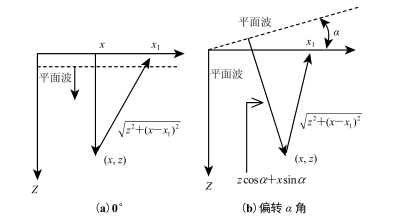
\includegraphics[width=0.8\linewidth]{principle1}
	\caption{Time delays for plane wave insonification}
	\label{fig:principle1}
\end{figure}
\begin{equation}
\small
t_{1}(x_{i},x,z) = z/c + \sqrt{(z^{2}+(x-x_{i})^{2})}/c
\end{equation}
\begin{equation}
\small
t_{2}(x_{i},x,z) = (zcos\alpha+xsin\alpha)/c + \sqrt{(z^{2}+(x-x_{i})^{2})}/c
\end{equation}

\end{frame}

\begin{frame}{Principles}{Functional ultrasound imaging of the brain}
%\begin{equation}
\centering
\small
$t_{2}(x_{i},x,z) = (zcos\alpha+xsin\alpha)/c + \sqrt{(z^{2}+(x-x_{i})^{2})}/c$
%\end{equation}
\vspace{0.2cm}
\begin{equation}
S(x,z,\alpha) = \displaystyle{\int RF[x_{1},t(x,z,\alpha)] dx_{1} }
\end{equation}
\begin{equation}
CI(x,z) = \sum_{i=1}^nS(x,z,\alpha_{i})
\end{equation}or
\begin{equation}
CI = \frac{1}{N}\sum_{i=1}^NS_{B}^{2}(t_{i})
\end{equation}
where $\alpha$ is the angle of deflection.\\ $CI$ represent final combined images.
\end{frame}
\begin{frame}{Principles}{Frame frequency comparison}
	The velocity of ultrasound in brain is about 1540m/s.
	\\
	Assume the imaging depth is 5cm\\
	If there are 15 angle of deflection\\
	\vspace{0.7cm}
	\small
	Multi-angle plane wave coherent composite imaging algorithm:\\
	$F_{flat} = 15400Hz$, \alert{$F_{compound} = 1026Hz$}
	\vspace{0.5cm}
	\\
	Traditional 128 - line focused ultrasound frame frequency: \alert{120Hz}
	
\end{frame}

\begin{frame}{Principles}{Image of the brain}
\includemedia[
label=some_dice,
width=1.0\linewidth,height=0.5\linewidth, % 16:9
addresource=video.mp4, 
transparent,
activate=pageopen,
passcontext,
flashvars={
	source=video.mp4
	&autoPlay=true % start playing on activation
	&loop=true
}
]{}{VPlayer.swf}

\end{frame}
\begin{frame}{Principles}{Activation map}
\centering
\alert{Basically - Pearson's correlation coefficient}\\
\large
$\rho_{XY} = \frac{Cov(X,Y)}{\sqrt{D(X)}\sqrt{D(Y)}}$
\pause
	\begin{figure}
		\centering
		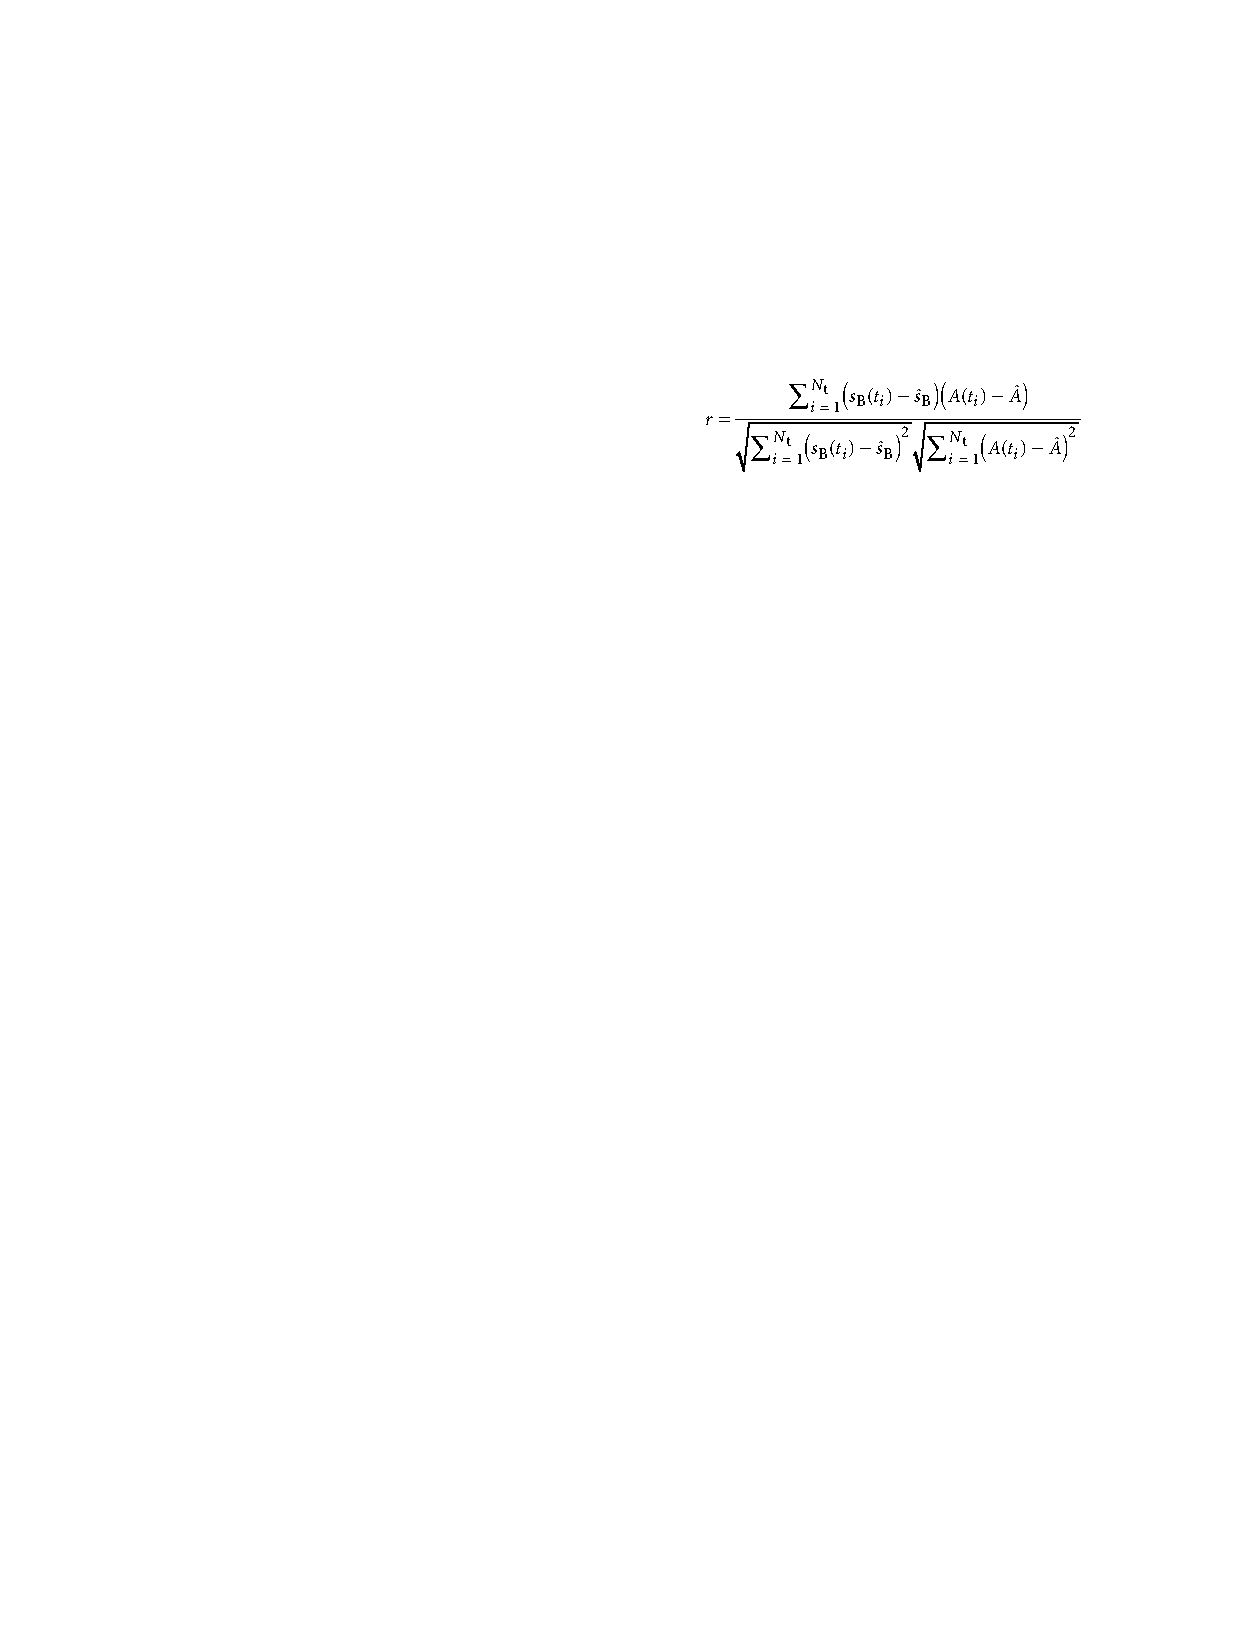
\includegraphics[width=1\linewidth]{formula}
	%	\caption{}
	%	\label{fig:formula}
	\end{figure}
	
$\left[
\begin{array}{ccc}
1\\
4\\
7\\
\end{array}
\right]$
$\left[
\begin{array}{ccc}
1\\
8\\
7\\
\end{array}
\right]$ = 0.7924
\end{frame}

\begin{frame}{Principles}{Video for Comparison}
\centering
\includemedia[
label=some_dice,
width=1\linewidth,height=0.5625\linewidth, % 16:9
addresource=UltrafastDoppler.mp4, 
transparent,
activate=pageopen,
passcontext,
flashvars={
	source=UltrafastDoppler.mp4
	&autoPlay=true % start playing on activation
	&loop=true
}
]{}{VPlayer.swf}
% loop video
\mediabutton[
mediacommand=some_dice:playPause,
overface=\color{blue}{\fbox{\strut Play/Pause}},
downface=\color{red}{\fbox{\strut Play/Pause}}
]{\fbox{\strut Play/Pause}}
\mediabutton[
mediacommand=some_dice:setSource [(UltrafastDoppler.mp4)]
]{\fbox{\strut Media Caption}}
\end{frame}







\subsection{Ultrafast ultrasound localization microscopy}
\begin{frame}{Optical super-resolution microscopy}{Inspiration from optical imaging}
\begin{figure}
	\centering
	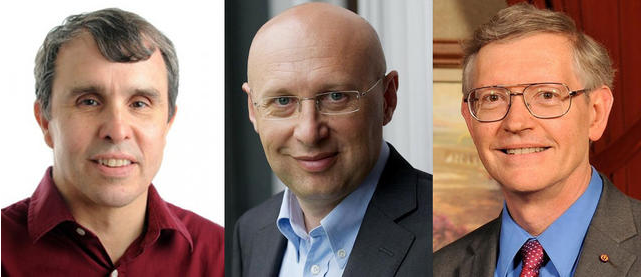
\includegraphics[width=0.8\linewidth]{noble}
	\caption{Winner of the 2014 Nobel Prize in Chemistry: \qquad \qquad \qquad (left) Eric Betzig, (middle) Stefan W. Hell, (right) W.E. Mona.
		\vspace{0.3cm}
		\centering
		\vspace{0.3cm}
		\alert{PALM}, STED, Photoactivation
	}
	\label{fig:noble}
\end{figure}
\end{frame}

\begin{frame}{Super-resolution ultrasound microscopy}{Tanter and his work}
\begin{figure} 
	\centering 
	\subfigure[Mickael Tanter]{ 
		%\label{fig:subfig:a} %% label for first subfigure 
		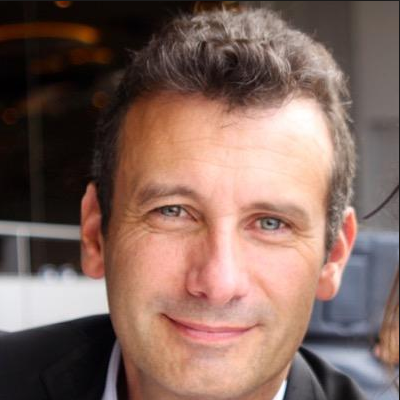
\includegraphics[width=1.5in]{tante} 
	} 
	\subfigure[Images of blood flow in the brain of rats by using superresolution ultrasound imaging method]{ 
		%\label{fig:subfig:b} %% label for second subfigure 
		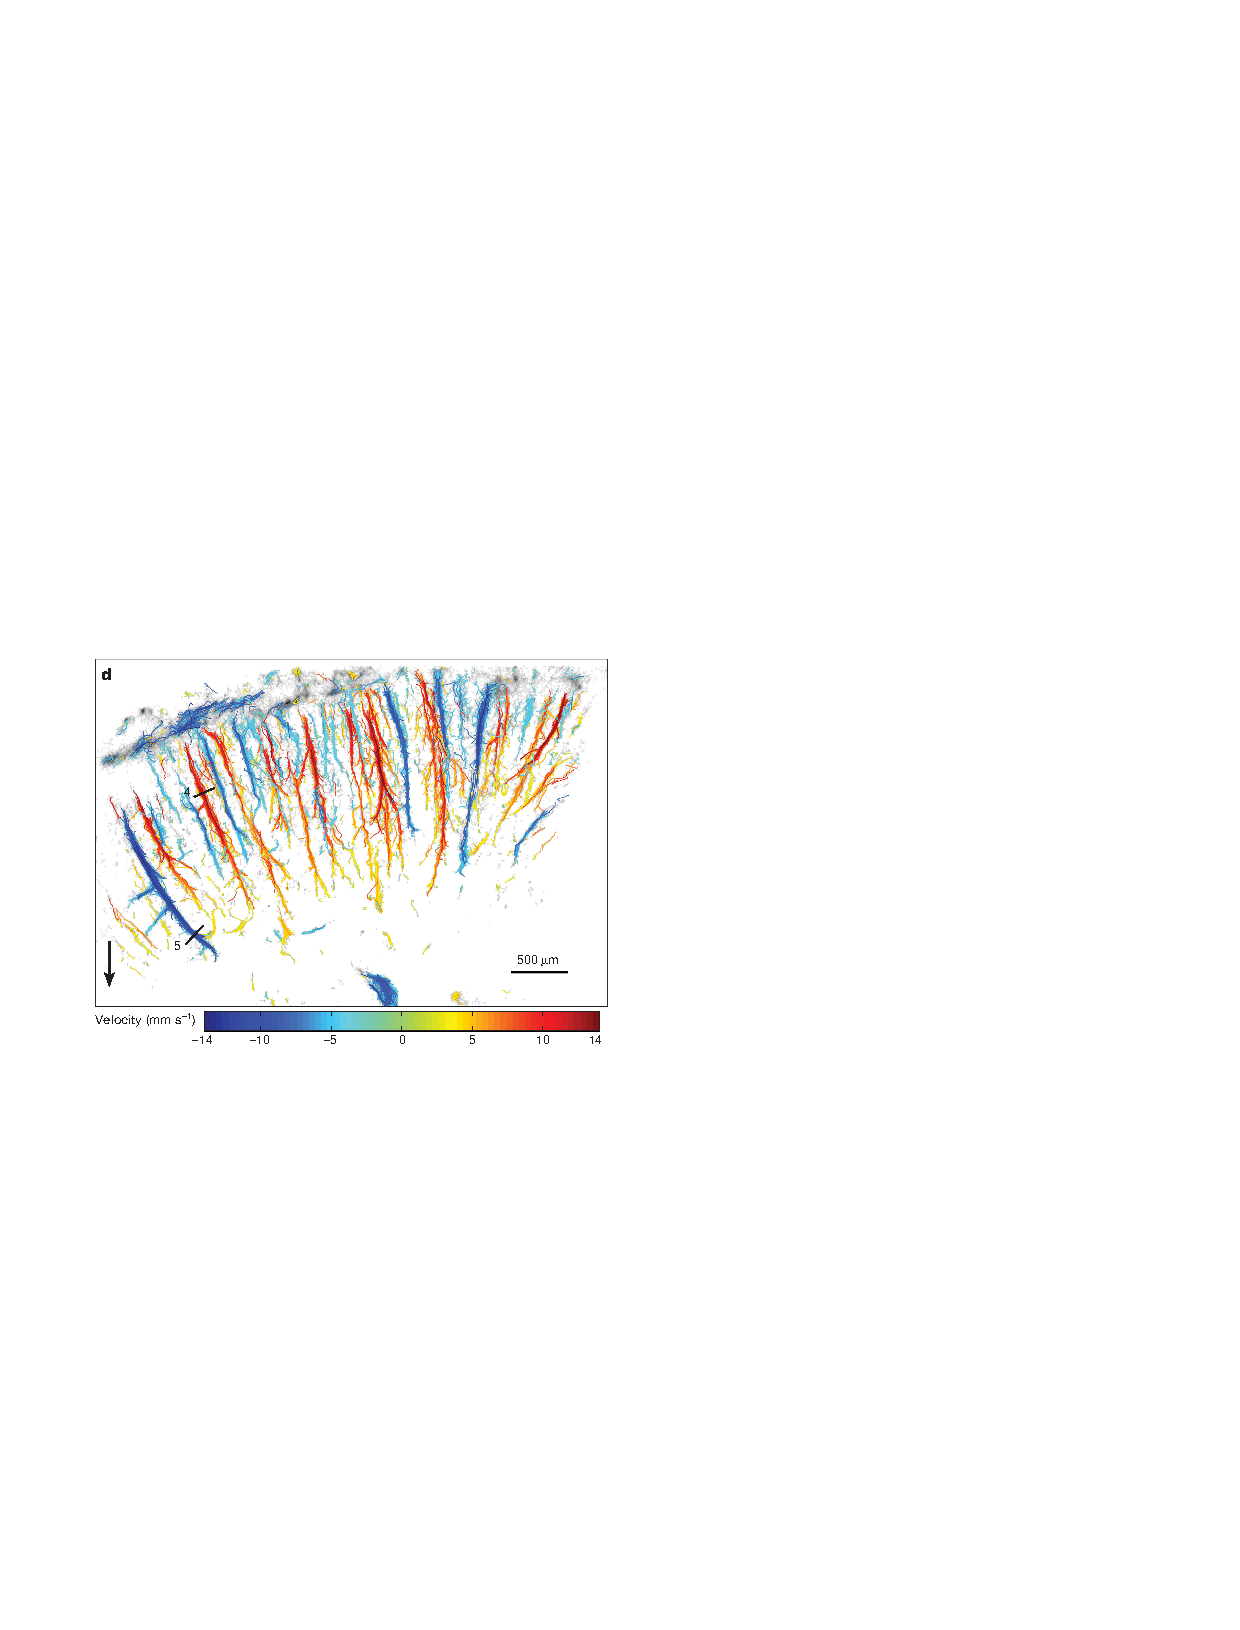
\includegraphics[width=2in]{need} 
	} 
	%\caption{Frames of the house and hotel data sets} 
	%\label{fig:subfig} %% label for entire figure 
\end{figure}
\end{frame}
\begin{frame}{Principles}{Airy disk}
\begin{figure}
	\centering
	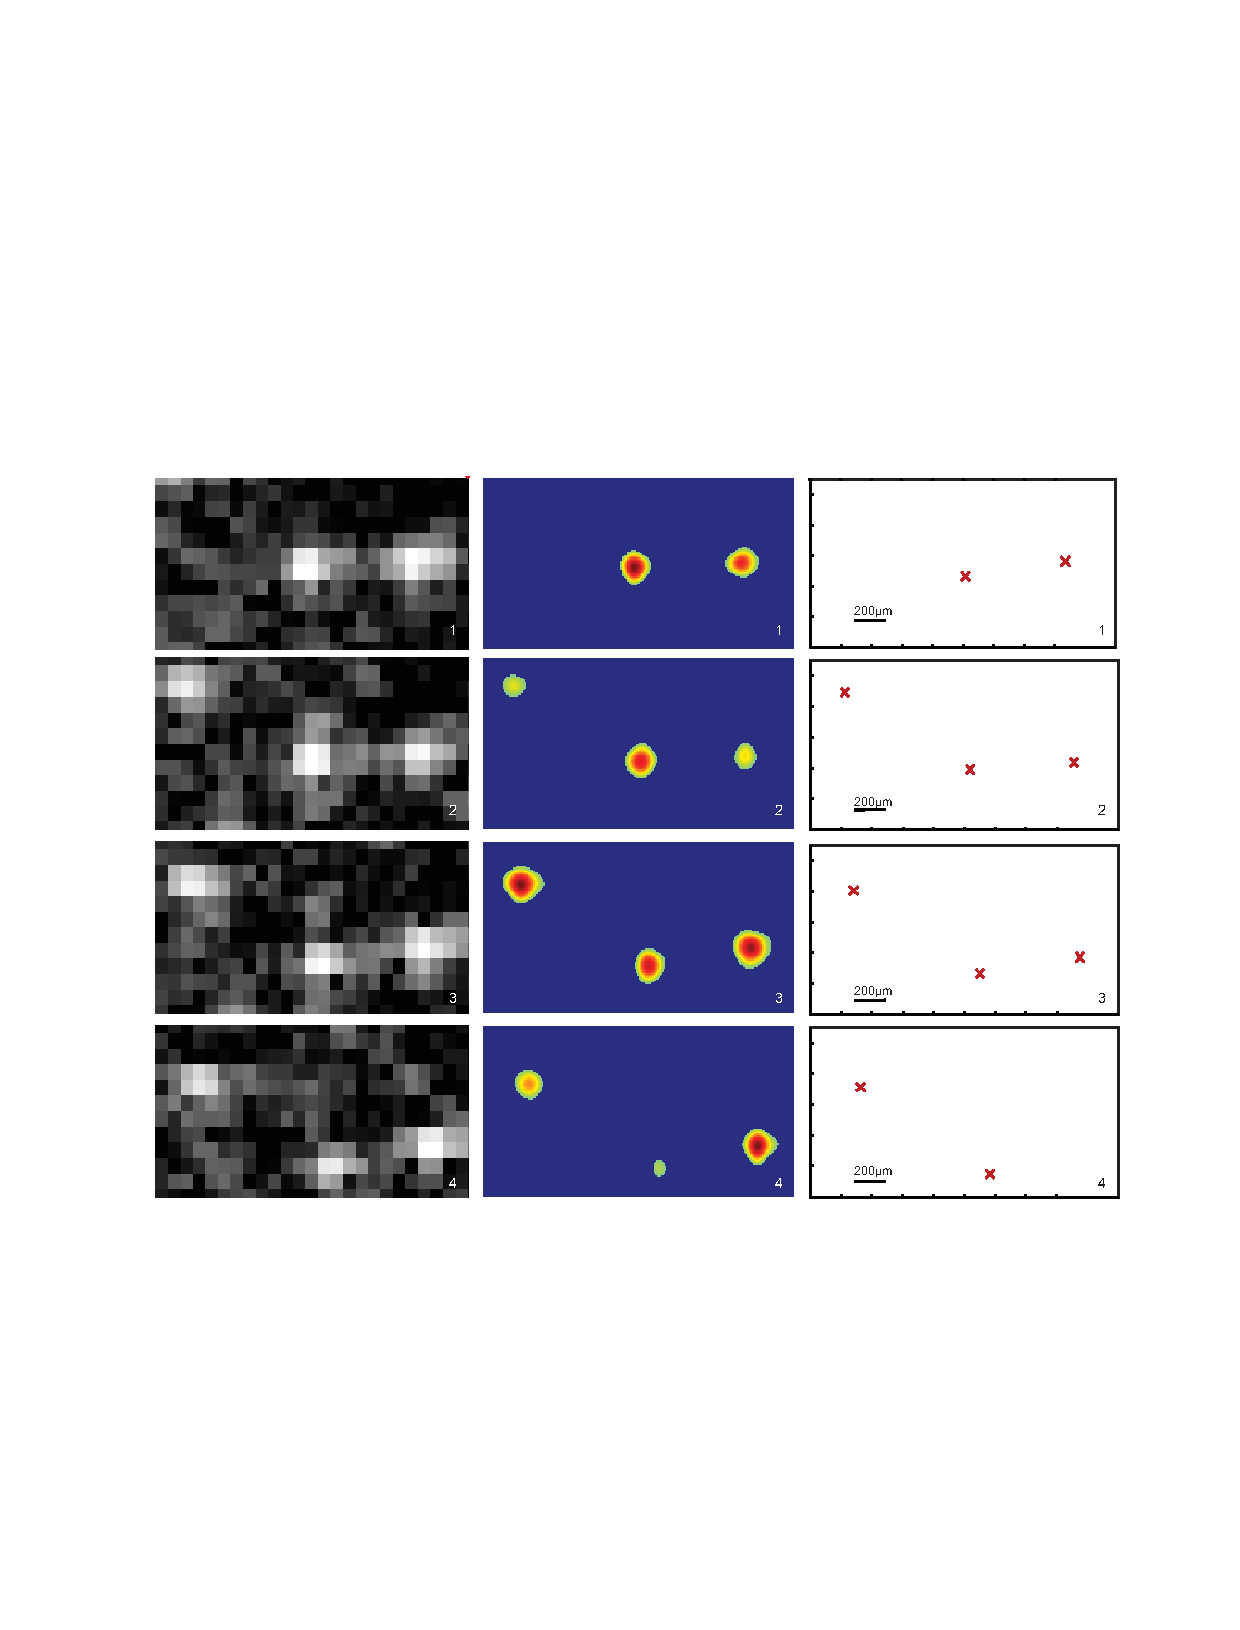
\includegraphics[width=0.8\linewidth]{need2}
	%\caption{}
	%\label{fig:need2}
\end{figure}
\end{frame}

\begin{frame}{Principles}{Bilinear interpolation}
	\begin{figure}
		\centering
		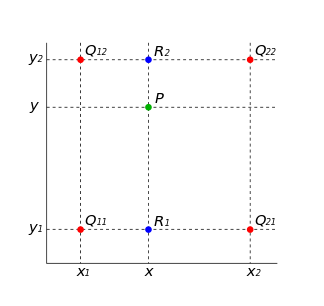
\includegraphics[width=0.75\linewidth]{bilinear}
		%\caption{}
		%\label{fig:bilinear}
	\end{figure}
\end{frame}

\begin{frame}{Principles}{Deep super-resolution vascular imaging}
\begin{figure}
	\centering
	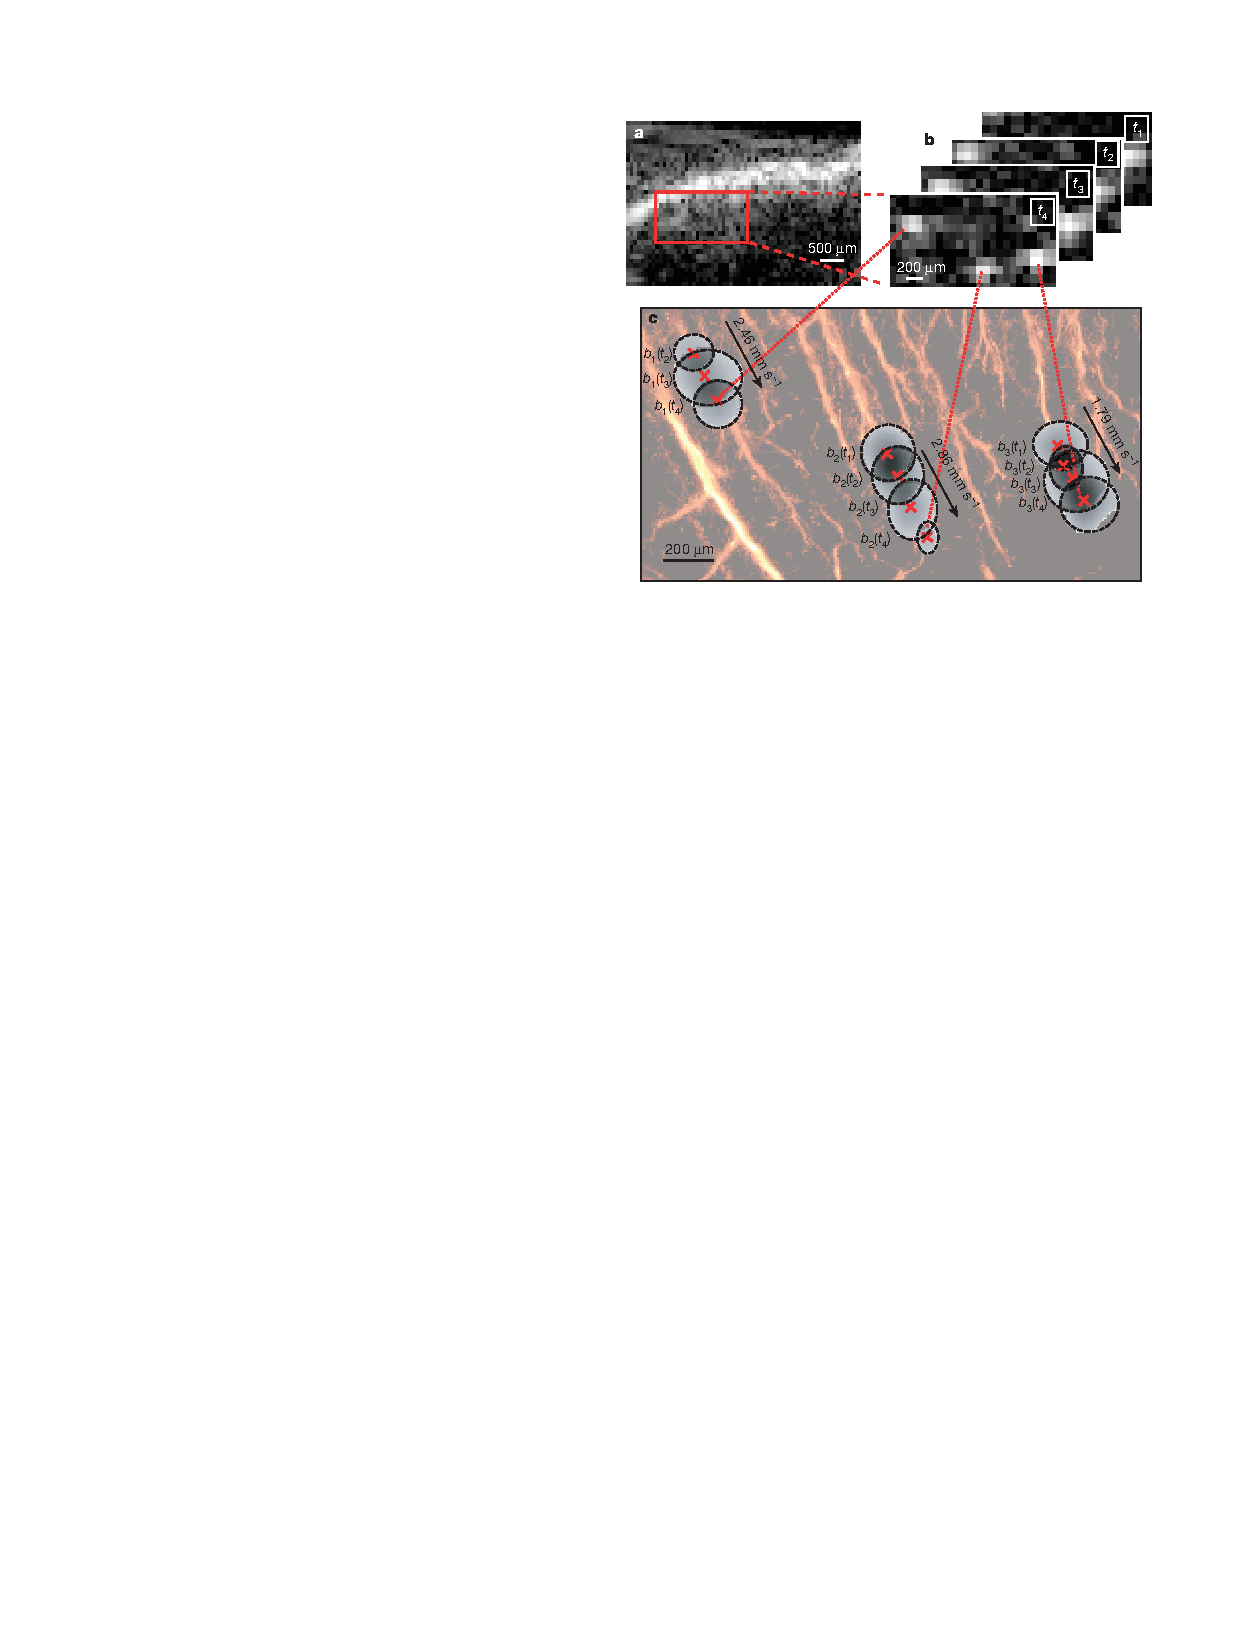
\includegraphics[width=0.75\linewidth]{fastimage}
	%\caption{}
	\label{fig:fastimage}
\end{figure}
\end{frame}




% You can reveal the parts of a slide one at a time
% with the \pause command:
\section{Application and prospect}
\subsection{Functional ultrasound imaging}
\begin{frame}{Comparison}{Functional ultrasound imaging}
  \begin{itemize}
  \item {
    Resolution ratio \& SNR
}
  \end{itemize}
\begin{figure}
	\centering
	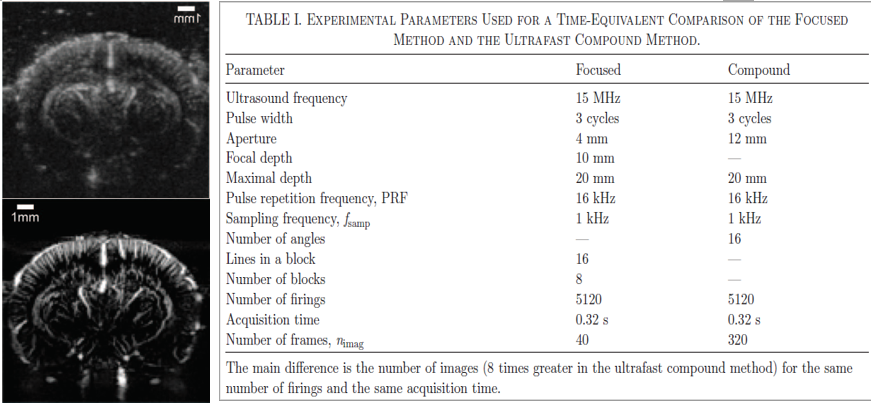
\includegraphics[width=1.05\linewidth]{im4}
%	\caption{}
%	\label{fig:im4}
\end{figure}

\end{frame}

\begin{frame}{Achievement}{Functional ultrasound imaging}
 \begin{itemize}
	\item {
		High temporal and spatial resolution
	}
	\vspace{1cm}
	\item{
	Good penetration depth
}
\end{itemize}
\end{frame}
\begin{frame}{Functional imaging in mobile small animal}
\includemedia[
label=some_dice,
width=1.0\linewidth,height=0.2\linewidth, % 16:9
addresource=RatHeader31.mp4, 
transparent,
activate=pageopen,
passcontext,
flashvars={
	source=RatHeader31.mp4
	&autoPlay=true % start playing on activation
	&loop=true
}
]{}{VPlayer.swf}\vspace{0.7cm}
Ultralight probes monitor brain activity in small animals
\end{frame}

\begin{frame}{Application and prospect}
\begin{block}{Neonatal pediatric neurology}
\begin{itemize}
	\item {
	Preterm infants seizures
}
\item{
Take the place of fMRI
}
\end{itemize}
\end{block}
\pause
\begin{block}{Functional ultrasound imaging in adults}
\begin{itemize}
	\item {
	Spatial localization of the activated area
}
\item{
Take the place of electrocortical stimulation mapping (ESM)}
\end{itemize}
\end{block}
\end{frame}
\subsection{Ultrafast ultrasound localization microscopy}
\begin{frame}{Comparison}
\alert{Question: capillary thickness}\\
\vspace{0.5cm}
May be a valuable tool for basic understanding and diagnosis of disease processes that alter microvascular blood flow
\end{frame}
\begin{frame}{Achievement}{Ultrafast ultrasound localization microscopy (uULM)}
\begin{itemize}
	\item {
High temporal and spatial resolution	
}
\vspace{1cm}
\item{
	The diffraction limit was broken ($\lambda$/10)
}
\end{itemize}
\end{frame}

\begin{frame}{Application and prospect}{Ultrafast ultrasound localization microscopy (uULM)}
	\begin{block}{Tumor}
		\begin{itemize}
			\item {
				Find tumor
			}
			\item{
				Know the growth of the tumor
			}
		\end{itemize}
	\end{block}
	\pause
	\begin{block}{Coronary microvascular disease}
		\begin{itemize}
			\item {
				Difficult to visually detect the disease
			}
			\item{
				Therapeutic effects cannot be directly quantified
			}
		\end{itemize}
	\end{block}
\end{frame}



% All of the following is optional and typically not needed. 
\appendix
\section<presentation>*{\appendixname}
\subsection<presentation>*{For Further Reading}

\begin{frame}[allowframebreaks]
  \frametitle<presentation>{For Further Reading}
    
  \begin{thebibliography}{4}
  \beamertemplatearticlebibitems
  % Followed by interesting articles. Keep the list short. 

  \bibitem{Functional Ultrasound Imaging of the Brain:
  	Theory and Basic Principles}
    Mace, E., Tanter, M., et al.
    \newblock Functional Ultrasound Imaging of the Brain:
    Theory and Basic Principles
    \newblock {\em IEEE Transactions On Ultrasonics, Ferroelectrics And Frequency Control, 60(3), 492-506. doi: 10.1109/tuffc.2013.2592}
    
    \bibitem{Ultrafast ultrasound localization microscopy for deep super-resolution vascular imaging}
    Errico, C., Tanter, M., et al.
    \newblock Ultrafast ultrasound localization microscopy for deep super-resolution vascular imaging
    \newblock {\em Nature, 527(7579), 499-502. doi: 10.1038/nature16066}
    
    \bibitem{Functional Ultrasound Imaging of the Brain}
    Mace, E., Tanter, M., et al.
    \newblock Functional Ultrasound Imaging of the Brain
    \newblock {\em Nature Methods, 8(8), 662-664. doi: 10.1038/nmeth.1641}
    \bibitem{Intraoperative Functional Ultrasound Imaging of Human Brain Activity}
    Imbault, M., Tanter, M., et al.
    \newblock Intraoperative Functional Ultrasound Imaging of Human Brain Activity.
    \newblock{\em Scientific Reports, 7(1). doi: 10.1038/s41598-017-06474-8}
  \end{thebibliography}
\end{frame}

\end{document}


